% !TEX TS-program = pdflatex
% !TEX encoding = UTF-8 Unicode

%************************************************
\chapter{La Composizione}
\label{chp:La Composizione}
%************************************************

Delineati i tratti "somatici" di Sp.I.R.E. ho potuto finalmente immergermi nella stesura di una composizione scritta \textit{ad hoc} per lo strumento. Tra i primi appunti c'era la stesura di una partitura che potesse legare tra loro:

\begin{itemize}
\item{il teatrale, dato che l'approccio e la fisionomia del nuovo oggetto-strumento porta anche a delineare nuove forme performative e compositive}
\item{Un nuovo mondo sonoro}
\item{L'interazione tra elettronica e microfoni tramite dei feedback indotti dai movimenti del pedale da parte del perfomer, quindi, filtri risonanti}
\item{Un elettronica costruita a misura che comprendesse: modulazione di frequenza e modulazione ad anello, per l'amore che mi lega a questi processi di sintesi}
\end{itemize}

\begin{wrapfigure}{r}{5cm}
\centering
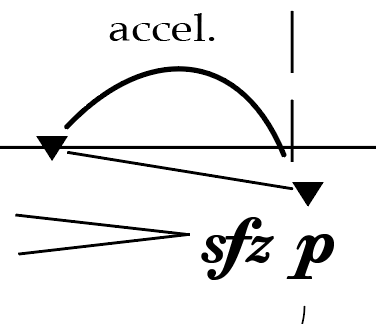
\includegraphics[width=.19\textwidth]{fig01.jpg}
\caption{particolare partitura \textit{Vitres de Son}}
\label{default}
\end{wrapfigure}

La struttura complessiva del brano è tripartita. Ogni parte è costruita su una quartina della poesia. Le righe della partitura si differenziano per piccoli tratti gestuali: ogni figura ha l'unione di uno o più timbri. In questo esempio, vediamo un pizzicato, dato dal simbolo triangolare\footnote{tutti i simboli verrano esplicati nella sezione dedicata alla legenda} e un glissato sulla molla, che produce uno strofinio (fig.10). 

L'insieme di più forme musicali sovrapposte per delineare un timbro complesso è una pratica cara al compositore Simone Santi Gubini. Durante la sua masterclass tenutasi al Santa Cecilia durante \textit{EMUFest 2017} ci spiegò che l'utilizzo di più tecniche sovrapposte, come in figura 11, rende possibile un'assimilazione veloce del gesto e una chiarezza di linguaggio. 

\begin{figure}[htbp]
\begin{center}
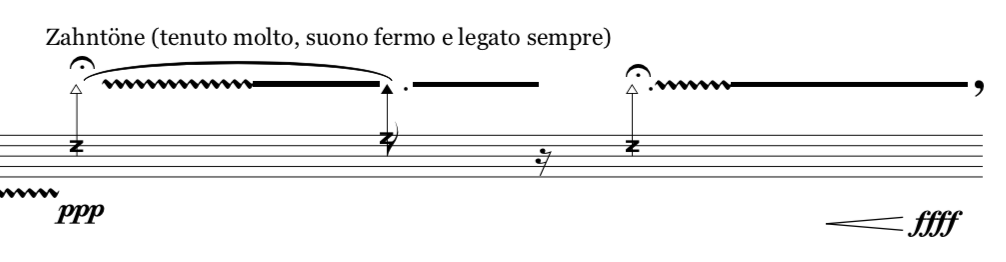
\includegraphics[width=.9\textwidth]{Gubini01.jpg}
\caption{Particolare partitura \textit{Klangrelief (Relief II)} di Simone Santi Gubini}
\label{default}
\end{center}
\end{figure}

%\begin{figure}{r}{5cm}
%\centering
%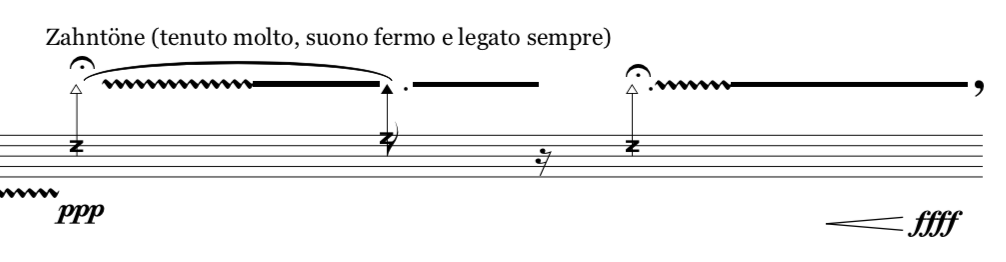
\includegraphics[width=.9\textwidth]{Gubini01.jpg}
%\caption{Particolare partitura \textit{Klangrelief (Relief II)} di Simone Santi Gubini}
%\label{default}
%\end{figure}

Così ho sfruttato tali insegnamenti per provare a sommare più simboli per arrivare ad un timbro complesso.
Tutte forme ritmiche appaiono più come dei gesti musicali che come cellule ritmiche vere e proprie e fanno acquistare al pezzo delle caratteristiche prosodiche, come se ogni piccola cellula reciti un verso della poesia.

%************************************************

\subsection*{I Parte}

L'incipit è dato da una forma distesa piena di frequenze basse che somigliano a dei rintocchi. Qui iniziano a prendere vita le prime cellule ritmiche, cercando di andare di pari passo con una lettura temporale della poesia di Artaud: dalla vista dal basso verso l'alto degli astri (\textit{verres où cuisent les cerveaux / le ciel fourmillant d'impudeurs}).

%************************************************

\subsection*{II Parte}

Ho congiunto le varie forme ritmiche con delle parti di soundscape creato grazie a un tremolo lento sulle molle più grandi. Tali macchie di suono rendono possibile lo sviluppo di un continuum che si manifesta in lontananza per riaffiorare in alcuni punti, decadendo poi velocemente, seguito da vertiginose corse delle dita sulle molle. Ogni cellula ritmica che si forma, si ripete, ma con piccole variazioni, ogni gesto è riconosciuto sia nella semiografia che dal timbro percepito. L'elettronica entra in sordina, si adagia nel sottosuolo dei pianissimo ed emerge a tratti (in contrappunto con i tremoli) sempre più delineati, fino a sfociare in un feedback controllato sul solo della Molla 5. 

%************************************************

\subsection*{III Parte}

Un piccolo intermezzo divide la parte II dalla III, un piccolo fraseggio che divide il solo dal continuum successivo. Il secondo continuum non è un passaggio di personaggio sonori (le molle), ma è l'evoluzione di gesti sulle lastre, che, da leggera patina sonora si trasformano in stridenti movimenti d'archetto che convogliano in jeté (\textit{un tourbillon d'ailes sauvages}) per sfociare definitivamente in arcate pesanti su lastre opposte fino al crescendo finale. La struttura della III parte è tutta una preparazione a questo crescendo che culmina in un pedale che Sp.I.R.E. possiede naturalmente.

Entrando nel merito della stesura compositiva, vado a sottolineare alcune peculiarità del movimento orizzontale e verticale delle voci.  o a leggeri passaggi di archetto, come si nota nella III parte della composizione. Tali macchie di suono, rendono possibile, nella II parte, lo sviluppo di un continuum, .

Le varie parti di modulazione di frequenza e le interazioni ritmiche si incastrano seguendo un movimento verso le frequenze più alte. la notazione si erige, come grande rosone, verso armoniche generate sia dal materiale metallico composto dalle molle, sia da quello delle piastre. Si va ad indagare, quindi, \textit{nello} strumento (tramite una scrittura prettamente legata all'universo delle percussioni) sia textit{sullo} strumento (tramite l'utilizzo dell'elettronica). Tengo a sottolineare che l'amplificazione è colonna portante di tutto il brano, dato che tutte le elaborazioni e i contributi dell'elettronica sono diffusi esclusivamente tramite gli attuatori. L'amplificazione e qualunque elettronica a supporto della performance sono amplificate dai piezoelettrici e dai microfoni omnidirezionali e cardioidi.

Ogni contributo elettronico è un valore \textit{intrinseco} a Sp.I.R.E. che lascia riecheggiare nell'ambiente circostante tutte le sue risonanze.

%************************************************

\section{Materiali sonori}

Vitres de son è stata composta quindi su un sistema che si può definire sia \textbf{Acustico} che \textbf{elettronico}\footnote{Acustica musicale e architettonica a cura di Sergio Cingolani, Renato Spagnolo UTET, 2004 Torino p. 3}.

Suoni di sfondo si adagiano su una superficie sonora o un sondscape o su un continuum o sulle sub-armoniche. Da qui, emergono piccoli grattati che si ingrastrano con le figure ritmiche, diventano protagonisti, dal paesaggio sonoro, da un soundscape fatto di piccoli grattati in \textbf{\textit{ppp}}, emergono e sillabe dei versi della poesia. Come se prendessero la forma di piccoli respiri dati dalla lettura delle parole del poeta. Appare un \textit{dramma}, un enorme piaga che sottolinea Artaud in tutta la sua poetica giovanile e nei suoi lavori teatrali: non c'è più linguaggio parlato, divincolato dalla struttura principale di diffusione orale, ma solo suono. Il finale è l'elettronica: musica come poesia.

Nello stesso modo con il quale si applicano modifiche a livello di velocità di emissione delle sillabe durante una recitazione, così ho cercato di dar vita a delle variazioni nelle strutture ritmiche che si fondo con l'universo sonoro sottostante e vengono inghiottite dal soundscape. Ciò è reso possibile dalla natura del materiale: ogni passaggio delle dita o unghie sulle spire delle molle crea dei micro-glissati che formano maglie di suono che si fondono con le elaborazioni del live electronics. Ad un tratto appare, su frequenze gravi, una modulazione di frequenza. Questa FM, al suo interno ha dei piccoli movimenti spettrali, legati ad altrettanto piccole variazioni di parametri interni. Come affermava Xenakis:

\begin{quotation}
Una moltitudine di brevi \textit{glissandi} può dare l'impressione del continuo, come anche una moltitudine di \textit{pizzicati}\footnote{Iannis Xenakis, \textit{Universi del suono, Scritti e interventi 1955-1994} (a cura di Agostino Di Scipio), Ricordi S.r.l. e LIM Editrice S.r.l., 2003}.
\end{quotation}

%************************************************

\section{Idea ritmico-melodica}

Ho cercato di creare una cellula di suoni disposti orizzontalmente, per poi lavorare sulla parte contrappuntistica. Dato che il nuovo strumento non ha \textit{pitch} definiti è stato complicato lavorare su una cellula che al finire del suo svolgersi si potesse definire conclusa. Difatti ho cercato degli stratagemmi musicali, come accenti o determinati effetti timbrici (ad esempio attivazione di armoniche sugli estremi delle molle) che potessero diventare dei gesti musicali, sia a livello grafico che d'ascolto. L'insieme di accenti o di un numero determinato di gesti, vanno a formare le cellule ritmico-melodiche che interagiscono con la materia di cui è composto lo strumento, sempre con un rapporto di 1:1 tra il ferro armonico delle placche e il metallo armoniche delle molle.
Sarà poi l'elettronica a legarsi agli accenti e agli incontri verticali delle varie cellule ritmico-melodiche. Si noti, durante la performance, che alcune scelte gestuali presenti in partitura, sono connesse ad un movimento esclusivamente performativo: quasi teatrale (ad es. l'incrocio degli archetti nella III parte).

Le figure ritmiche servono a dare alla composizione un andamento strutturale. Ovvero, anche se molte figure non sono legate ad un preciso \textit{ictus}, servono comunque a creare degli incontri, ad esempio tra elettronica e parte strumentale o il movimento verticale di più voci. in \textit{Vitres de Son} in queste figure ritmiche sono nascoste le sillabazioni dei versi della poesia di Artaud, cercando di far intuire un andamento "vocale" delle parti (fig. 6).

%\begin{figure}[htbp]
%        \centering
%        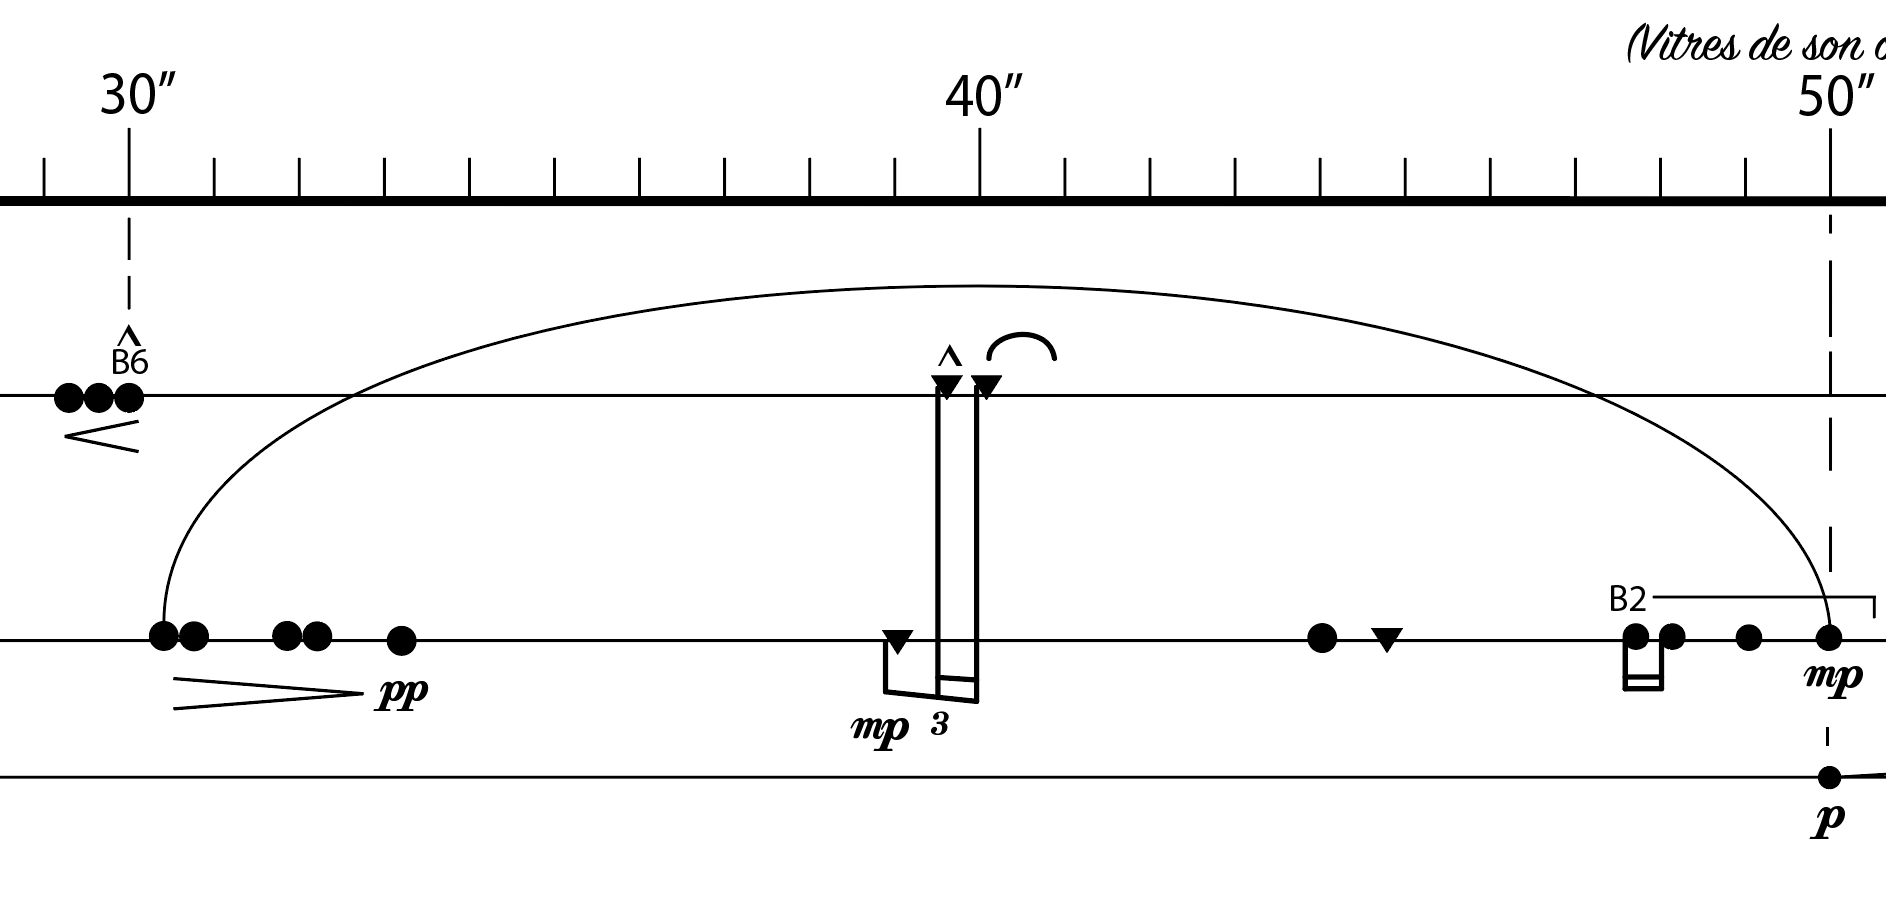
\includegraphics[height=15cm, width=15cm, angle=0,
%          keepaspectratio]{sillabaritmica.jpg}
%          \small{\caption{\textit{fraseggio ritmico}}}
%\end{figure}

\begin{figure}[htbp]
\begin{center}
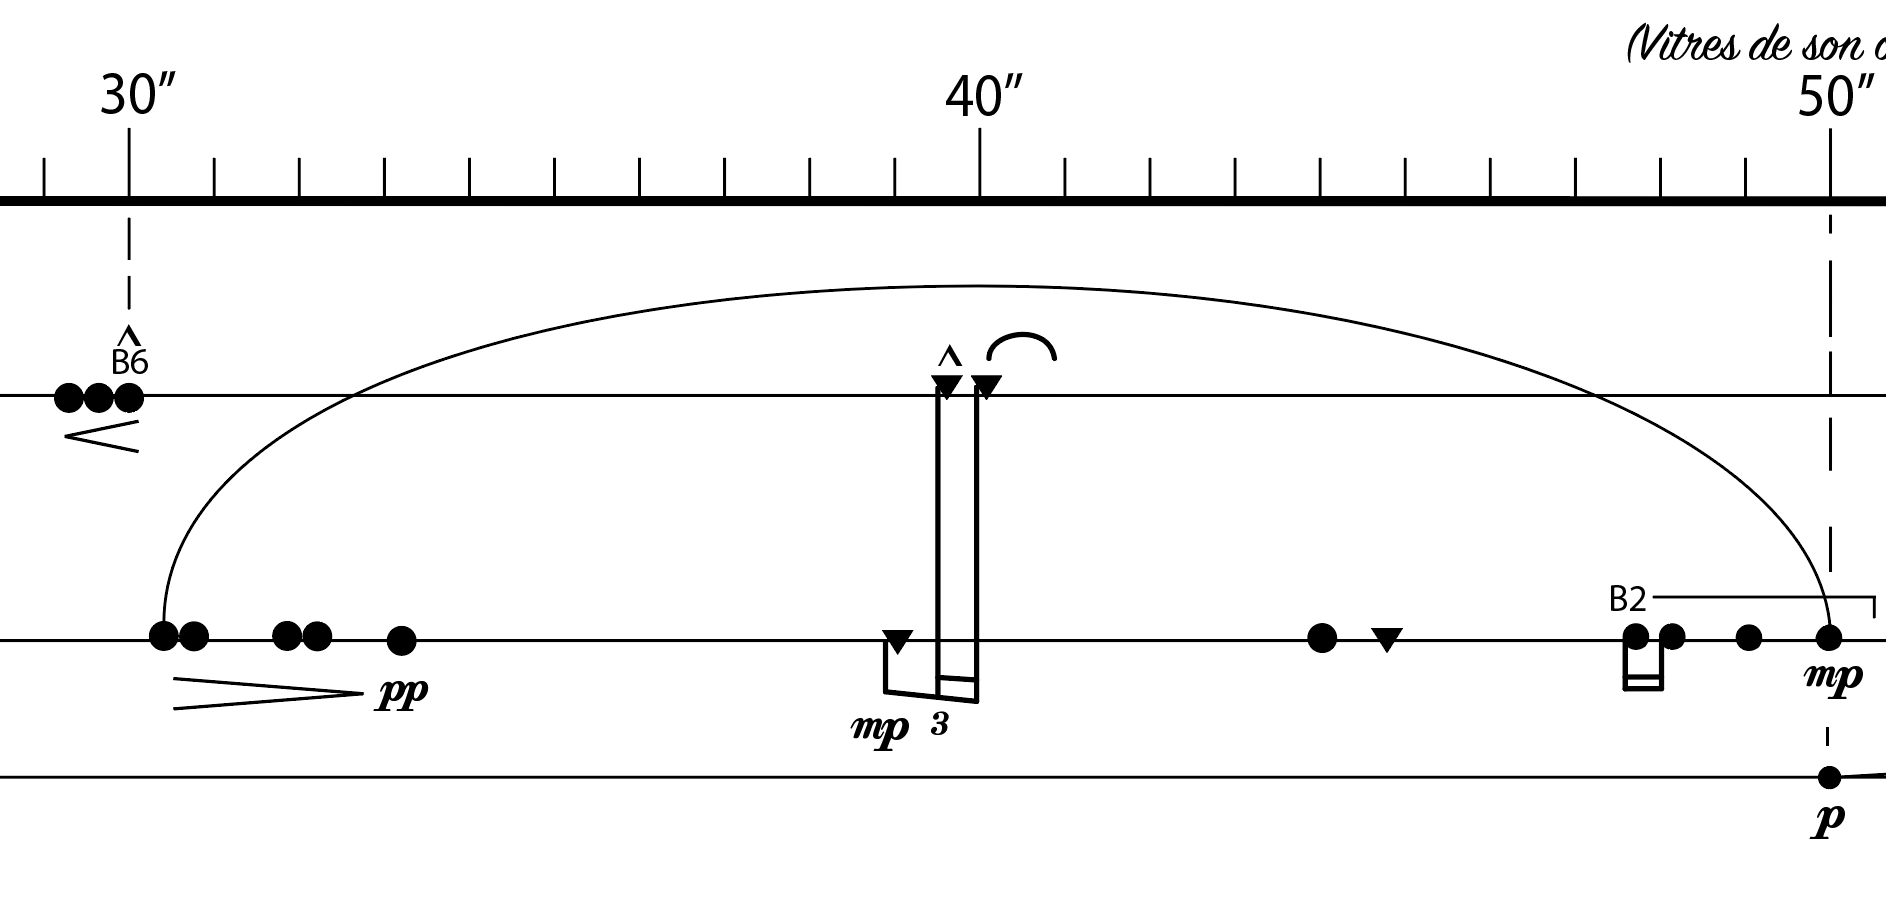
\includegraphics[width=.99\textwidth]{sillabaritmica.jpg}
\caption{fraseggio ritmico}
\label{default}
\end{center}
\end{figure}

Ho considerato utili tecniche di scrittura contemporanea legate al mondo degli idiofoni e all'universo dei cordofoni.

Per quanto riguarda la notazione, ho trovato, nel libro sulla semiografia contemporanea di Luigi Donora\footnote{Luigi Donora, \textit{Semiografia della nuova musica}, }, molte delucidazioni sulla creazione di figure ritmiche e simboli che potessero al meglio rappresentare il mio fine compositivo. Per fine compositivo intendo la possibilità di creare determinati timbri, riportando notazioni non canoniche ma che facessero capire la tipologia di gesto da utilizzare in un determinato frammento. Durante la stesura della partitura ha cambiato forma diverse volte. La prima partitura, infatti, era stata creata direttamente su una serie di pentagrammi, dove il si sopra al do centrale stava a simboleggiare il centro della molla e il movimento verso l'alto e verso il basso delle note rappresentava rispettivamente un movimento verso destra e verso sinistra (fig. 7)
Ogni cellula si sovrappone poi ad altre cellule simile in piccoli inserti contrappuntistici fatti di dilatazioni o restrizioni temporali del materiale sonoro.

A livello compositivo compaiono delle cellule ritmiche che vanno a confluire in grossi nubi sonore. L'attinenza tra la scrittura e il gesto a volte è slegata, ma le piccole note e la tendenza ad una continuità notazionale porta l'esecutore-performer a capire in quali punti vanno gestiti dei continuum.

Le figure ritmiche servono a dare alla composizione un andamento strutturale. Ovvero, anche se molte figure non sono legate da un ictus preciso, servono comunque a creare degli incontri, tra elettronica e parte strumentale o in alcuni punti nell'incontro verticale di più voci. All'interno di queste figure ritmiche sono nascoste le sillabazioni dei versi della poesia di Artaud che prende il nome del pezzo e rendono possibile una vocalità dei movimenti ritmici.

Ho considerato utili tecniche di scrittura contemporanea legate al mondo degli idiofoni e all'universo dei cordofoni. Per quanto riguarda il pentagramma, nella prima stesura era stato utilizzato per il movimento sulle corde, come in figura, si identifica il movimento da sinistra verso destra, con il movimento dal basso verso l'alto. In seguito, ogni movimento sul pentagramma, ogni forma che produceva un suono differente, si è trasformata in simbolo: ogni simbolo rappresenta quindi un gesto che si sviluppa in un determinato suono con un suo timbro specifico.
Saranno considerate utili tecniche di scrittura contemporanea, legata al mondo delle percussioni per lo strumento di nuova creazione. Il pentagramma diventa la base di un movimento sull'asse orizzontale dello strumento. Il pentagramma con centro sul Si sopra al Do centrale, nella prima stesura, ed un uno rigo unico con centro nel rigo stesso nella seconda, rappresentano graficamente una determinata molla che sarà nominata in legenda con la lettera M. Per rendere più semplice ogni movimento e ogni incastro ritmico, ho redatto degli esempi che vengono esplicati in legenda tramite una didascalia, così da migliorare l'approccio con la partitura e con l'iper-strumento.

\section{Gestualità}

%\begin{wrapfigure}{r}{5cm}
%\centering
%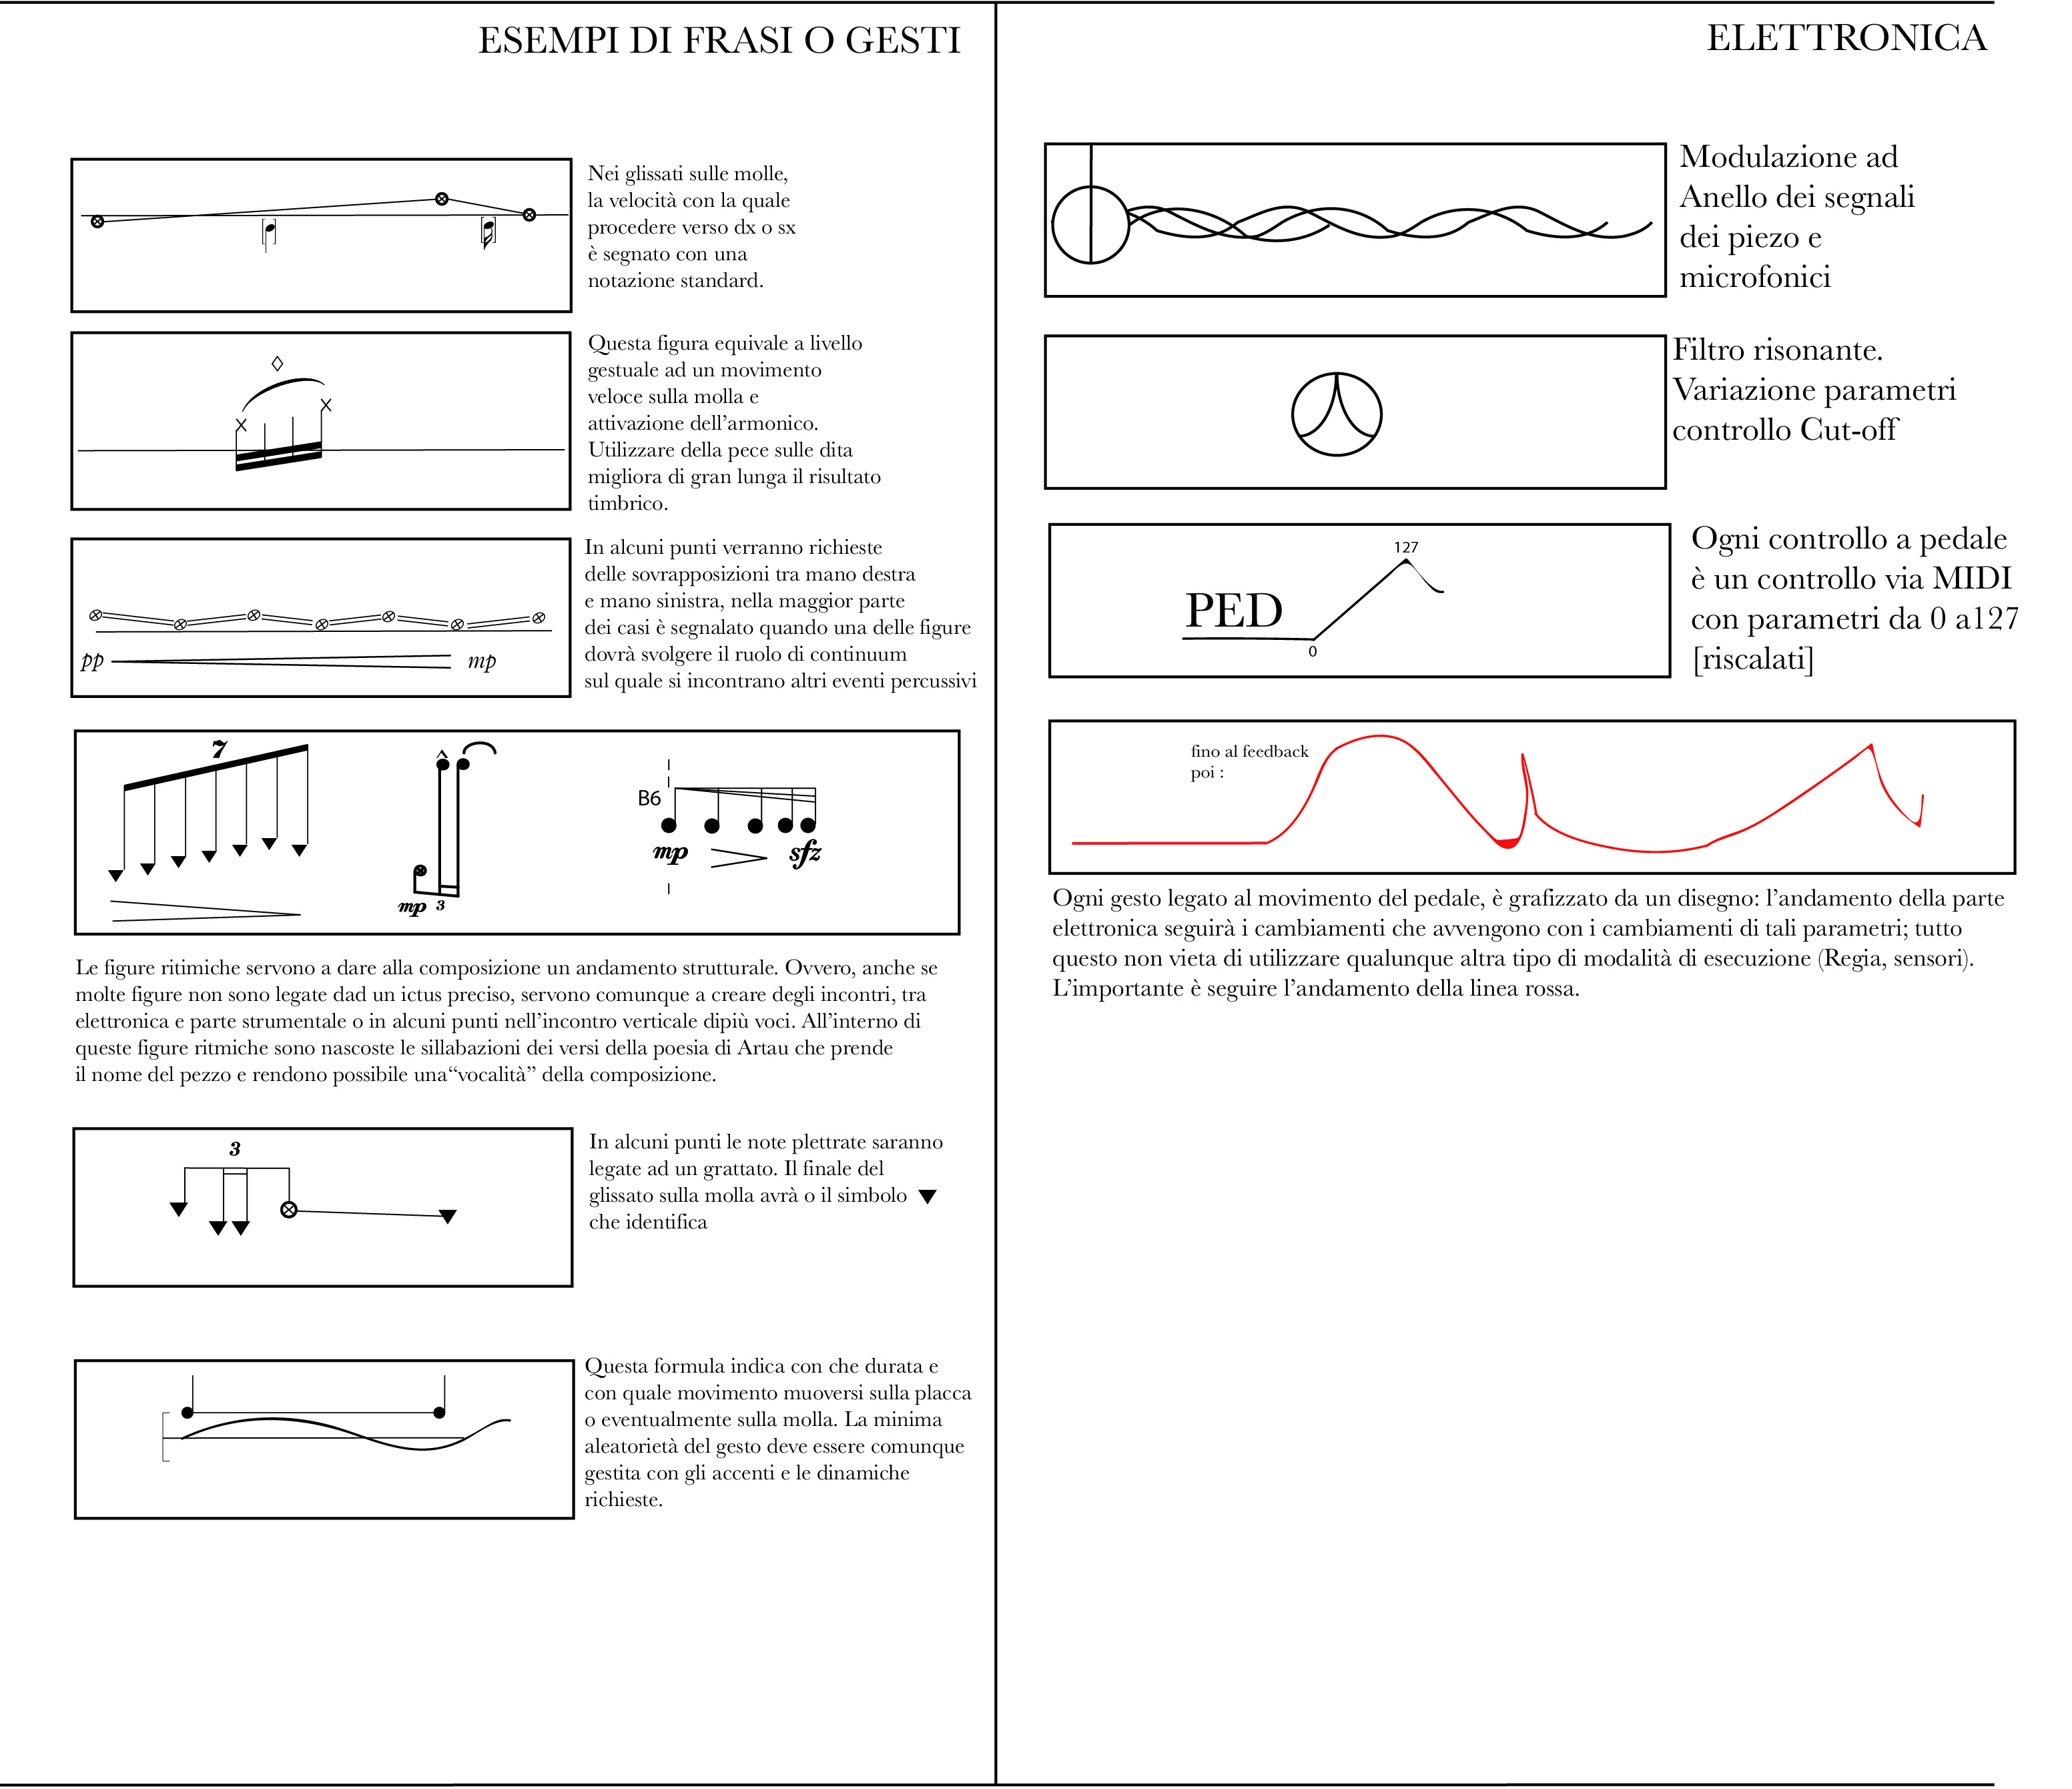
\includegraphics[width=.29\textwidth]{legenda2.jpg}
%\caption{default}
%\label{default}
%\end{wrapfigure}

La fortuna di questo strumento è che per metà è acustico e che è in alcuni casi ha una curva di decadimento molto larga.
La puntualità in partitura nel far capire quali punti della molla colpire è alla base di un gesto preciso, che possa essere sempre lo stesso per lo stesso simbolo scritto e per la stessa risultante sonora. La legenda, quindi, oltre ad avere l'esplicazione della simbologia, ha anche dei piccoli esempi di qualche rigo della partitura o dell'utilizzo del pedale; in alcuni casi può risultare estremamente efficace per migliorare l'esecuzione del brano.

\clearpage

\thispagestyle{empty}

\includepdf[offset=-30 10,
		    scale=1.,
		    pagecommand={
		    	\begin{tikzpicture}[
					remember picture,
					overlay]
		    	\node [xshift=10cm,yshift=1cm] at (current page.south west) {\color{white}{}};
				\end{tikzpicture}}
		    ]{Macroforma01.pdf}

\clearpage

Continuando l'analisi della partitura, notiamo che ha, come oggetto principale di scrittura, il processo con il quale sono stati ricercati i suoni: ogni simbolo grafico rappresenta un gesto. Non viene perciò rappresentata la risultante timbrica, ma piuttosto il processo con il quale si va a produrre un determinato suono. Sarà, quindi, il gesto ad essere la base della prosodia interna, ogni legame con il gesto successivo sarà studiato per dare sia un movimento alle voci, che possono essere sino a 3 simultanee (come si nota nel solo sulla molla 5), sia per dare una sensazione di continuum. \\
L'utilizzo di simboli vicini al mondo della musica classica mi ha aiutato ad adeguare uno strumento del quale non abbiamo letteratura verso una nuova scrittura. Questo procedimento è la base poi della musica contemporanea, ovvero, ogni nuovo gesto è la decodifica di un simbolo evoluzione di musica più antica. \\
Alcuni movimenti scritti per l'archetto, infatti, stanno a simboleggiare un gesto, come avveniva in passato per la musica gregoriana, con i \text{melismi} legati al movimento delle mani del direttore di canto gregoriano.
\begin{figure}[!h]
\begin{center}
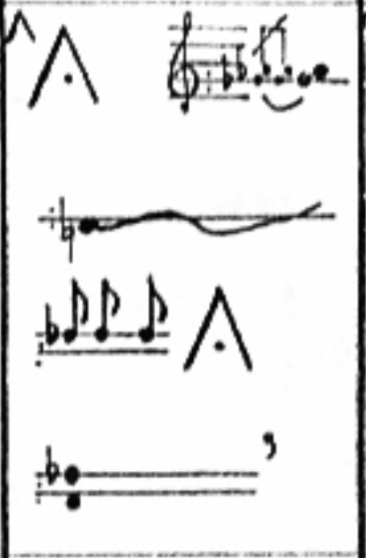
\includegraphics[width=0.19\textwidth]{guaccero01.jpg}
\caption{\textit{Particolare di Sinfonia 1 di Domenico Guaccero}}
\label{default}
\end{center}
\end{figure}
\section{Macro-forma}

Forma tripartita. dall'alto in basso: figure ritmiche, soundscapes ed elettronica.

\section{La legenda}
La partitura si apre con il progetto di Sp.I.R.E., per poterlo riprodurre ed utilizzare materiali affini.\\
Per facilitare la lettura della partitura elettroacustica, ho preferito dividere la legenda in quattro blocchi fondamentali:
\begin{itemize}
\item{Il primo blocco comprende la tipologia di battenti, utilizzati anche nella musica classica, ma \textit{numerati}, per facilitare i cambi in partitura, dato che per ogni battente abbiamo un'eccitazione diversa delle molle e un timbro differente.}
\item{Il secondo blocco delinea la notazione e la simbologia presente in partitura}
\item{Il terzo blocco ha al suo interno degli esempi che facilitano lo studio degli incastri ritmici}
\item{L'ultimo blocco comprende tutti i simboli e i gesti legati all'elettronica (pedali, variazioni di parametri, elaborazioni)}
\end{itemize}

\clearpage

\thispagestyle{empty}

\includepdf[offset=0 0,
		    scale=0.9,
		    pagecommand={
		    	\begin{tikzpicture}[
					remember picture,
					overlay]
		    	\node [xshift=10cm,yshift=1cm] at (current page.south west) {\color{white}{}};
				\end{tikzpicture}}
		    ]{legenda2.pdf}

\clearpage

\clearpage

\thispagestyle{empty}

\includepdf[offset=-10 0,
		    scale=1.,
		    pagecommand={
		    	\begin{tikzpicture}[
					remember picture,
					overlay]
		    	\node [xshift=10cm,yshift=1cm] at (current page.south west) {\color{white}{}};
				\end{tikzpicture}}
		    ]{legenda3.pdf}

\clearpage

\section{Algoritmi}

Tutti gli algoritmi sono stati disegnati prendendo ad esempio la simbologia esplicata da Walter Branchi nell'appendice 6 del libro \textit{Tecnologia della musica elettronica}\footnote{Walter Branchi, \textit{Tecnologia della musica elettronica} (con prefazione di Domenico Guaccero), Lerici, Roma, 1977}. Lo schema completo presente in partitura è vicino ad una visione sia di riproducibilità, che di visione globale, nella quale si intravede, già nello schema algoritmico il pensiero compositivo che c'è sotto.

Tecniche di sintesi utilizzate:

\begin{itemize}
\item{Sintesi Granulare, 8 voci}
\item{Modulazione di frequenza, 12 voci}
\item{Modulazione di ampiezza}
\item{Modulazione ad anello}
\item{Filtro Risonante}
\end{itemize}

\clearpage

\thispagestyle{empty}

\includepdf[offset=5 0,
		    scale=.90,
		    pagecommand={
		    	\begin{tikzpicture}[
					remember picture,
					overlay]
		    	\node [xshift=10cm,yshift=1cm] at (current page.south west) {\color{white}{}};
				\end{tikzpicture}}
		    ]{Algoritmica.pdf}

\clearpage

\section{Pedaliera}

Dopo aver studiato il funzionamento della pedaliera, ho notato che ogni pulsante numerato era assegnato ad un NOTE on, come una normalissima pedaliera midi per organo. La fortuna è che ogni pulsante equivale a note inerenti al numero presente sulla pedaliera (es. note-on 1 = tasto 1 pedaliera). Quindi essendo identiche, ho solo dovuto trasformare ogni note-on in un "lancio-scena" sul mio software di utilizzo (max-msp). Questo mi ha facilitato lo studio con il performer che poteva riprovare ogni scena senza doverle ripetere in sequenza temporale: ovvero poteva passare dalla scena 1 alla scena 6 senza dover ripercorrere tutte le scene presenti tra quelle menzionate. Questo ha facilitato di gran lunga le prove fatte per ogni singolo rigo.
